\documentclass[a4paper,10pt]{article}

\usepackage{ucs}
\usepackage[utf8]{inputenc}
\usepackage[francais,french]{babel}
\usepackage{fontenc}
\usepackage{graphicx}

\usepackage{fullpage}
\usepackage{amsmath}

\usepackage[dvips]{hyperref}
\usepackage{amssymb}

\newcommand{\coqcode}[1]{\texttt{#1}}

\date{10 novembre 2009}
\title{Rapport d'avancement du projet Coquille à mi-parcours}
\author{M1 Informatique Fondamentale ENS Lyon}

\begin{document}

\maketitle
\newpage
\section{Introduction}

\subsection{Présentation générale}

L’objectif de Coquille (« Coq User-Interactive Library Learning Expert »),
  est la réalisation d’un environnement de démonstrations de preuves mathématiques proche du monde des classes préparatoires. 
Il doit être élaboré à partir de l’assistant de preuves Coq. 
L’objectif est en somme d’élargir la portée de Coq au mathématiques de classes préparatoires,
 et à des mathématiciens non forcément experts en calcul des constructions et en théorie des types.

\subsection{Motivation}

La preuve assistée par ordinateur ouvre aux mathématiques de nouvelles perspectives. 
L'exemple le plus connu est la démonstration en Coq du théorème des quatre couleurs.  
Ce théorème n'a jamais été démontré sans l'usage de l'ordinateur.
 Même si pour l'instant, il y a très peu de théorèmes à avoir été démontrés d'abord en Coq, 
on peut espérer qu'en améliorant le langage de preuve, les bibliothèques de théorèmes et de tactiques, et en rendant Coq plus facile à utiliser,
 démontrer un théorème sera plus facile en Coq. 
Cela révolutionnera la façon de faire des mathématiques. Nous voulons apporter notre pierre à cet édifice.

En classes préparatoires, les élèves sont confrontés à un grand nombre de problèmes souvent répétitifs et non triviaux qui n'ont pas toujours 
de corrigés. Avoir un logiciel qui résoudrait le problème et donnerait sa démonstration permettrait d'avoir une correction automatique.
Nous voulons réaliser un tel logiciel.

\subsection{Public visé}

Nous souhaitons avant tout fournir un outil utilisable dans le contexte des classes préparatoires, 
mais il serait très fortement envisageable de le diffuser dans le monde de l'industrie et de la recherche 
(par exemple pour aider à confirmer des conjectures ou même des preuves lourdes en calculs et apporter une surcouche de fiabilité aux chercheurs)

\subsection{Approche}

La résolution devra être la plus automatique possible. 
Mais, les problèmes pouvant être difficiles, il n'est pas exclu que l'ordinateur demande de l'aide à l'utilisateur par moments.

Le logiciel doit être ergonomique: même si le public visé est assez scientifique pour vouloir prouver un théorème de mathématiques, il n'est pas forcément informaticien.

Nous souhaitons proposer à l'utilisateur un certain nombre de tactiques de haut niveau, correspondant aux différents chapitres du programme des classes préparatoires. Il sera nécessaire de mettre aussi à disposition des bibliothèques de preuves pour chaque chapitre.
Il y aura toujours deux versions pour chaque chapitre :
\begin{itemize}
    \item la version que l'on aura directement codée, stable.
    \item la version issue de l'apprentissage, qui continuera de s'améliorer au fur et à mesure que l'usager utilisera le logiciel.
\end{itemize}

Pour parvenir à ce résultat, ce projet de recherche s’est constitué autour de quatre groupes de travail :

\begin{itemize} 
\item Le groupe de travail IDE, concevant l'environnement de programmation
\item Le groupe preuves et tactiques, ayant pour but de faire une bibliothèque de théorèmes et de tactiques
\item Le groupe apprentissage, qui a partir de nombreux exercice résolu, génère automatiquement une tactique permettant de résoudre ce type d'exercice
\item Le groupe communication, facilitant la communication entre les groupes et diffusant COQUILLE aux potentiels utilisateurs
\end{itemize}

\subsection{Ressources Humaines :} 

Ce projet est développé par 22 élèves du M1 Informatique Fondamentale de l’ENS Lyon. 
Les tâches se sont réparties entre 4 Work Packages (WP) dont nous allons décrire l'avancement à mi-parcours. 
(Liste des participants et découpage des groupes de travail en annexe). 
Les WP se réunissent toutes les semaines: une heure séparés ainsi qu'une heure de mise en commun.

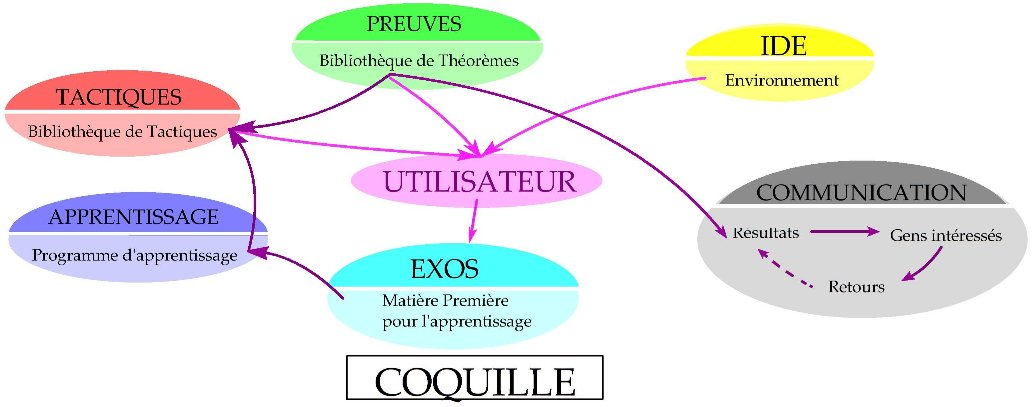
\includegraphics[scale=0.6]{organisation.jpg}

\section{Workpackage Communication}
\paragraph{Dirigé par Mathieu Barthelemy}, 5 participants

\subsection{Objectifs}
L'objectif de ce groupe de travail est de faciliter la coordination des autres groupes de travail et de promouvoir le projet et ses résultats auprès de potentiels utilisateurs.


\subsection{Matériels et méthodes}
Pour atteindre ces objectifs ce groupe de travail a réalisé un site internet [3]. Ce site rassemble: un forum [4] et un wiki [5] pour faciliter la communication interne,
 une présentation du projet et nos résultats les plus impressionnant pour attirer les utilisateurs, une page de contacts et la documentation de Coquille
 pour faciliter son utilisation.
Ce groupe a par ailleurs réalisé la rédaction des différents rapports hebdomadaires et coordonné la rédaction du rapport de mi-projet. 
Enfin, des documents de communications internes et des formations HTML et Latex ont par ailleurs été réalisés.


\subsection{Perspectives}
Ce groupe de travail prévoit de rendre la documentation disponible sur le site internet, pour tenir compte de l'avancée des WP.
 Il prévoit aussi de réaliser le rapport final et de préparer une démonstration du projet.
 Il est prévu de rendre le site plus interactif en permettant la mise à jour automatique de la documentation.
 Il est prévu de faire connaître Coquille en dialoguant sur des forums ou avec des utilisateurs potentiels.

\subsection{Résultats}
Les principales réalisations de ce groupe de travail sont le site internet [3] et le présent rapport.

\section{Workpackage Preuves et tactiques}

\paragraph{Dirigé par Pierre-Marie Pédrot et Marthe Bonamy}, 9 participants

\subsection*{Objectifs}
Le but de ce groupe de travail est d'établir une liste de théorèmes vus en classes préparatoires dans les domaines suivant: l'algèbre, l'analyse, la topologie et l'arithmétique.
Dans un deuxième temps l'objectif est de les formaliser en Coq pour les implémenter. Enfin le dernier objectif est de proposer des tactiques évoluées d'aide aux prouveurs. 


\subsection*{\'Etat de l'art}
Différents domaines mathématiques ont commencé à être formalisés en Coq[1,2], mais relativement succintement, et la quasi-totalité des formules que l'on voit dans les cours de classes préparatoires en sont absentes. 

\subsection*{Matériels et méthodes}
Dans un premier temps, des livres de classes préparatoires ont été parcourus afin de connaître les structures classiques des problèmes. Dans un deuxième temps, ce groupe est en train d'écrire les preuves en coq à partir du cours.
Afin d'être fidèle aux d\'emonstrations attendues, la logique classique est utilisée lorsque les théorêmes le requiert. Nous avons toutefois essayé de limiter au maximum son utilisation.

Ce groupe de travail réutilise la librairie standard, au besoin et en l'étendant. 

% Pour la partie tactiques, le langage utilisé est évidemment ltac. 


\subsection{Logique}

\subsubsection{Indénombrabilité de $\mathbb{R}$ (\coqcode{Runcountable})}

\paragraph{Motivations}

Le résultat d'indénombrabilité de $\mathbb{R}$ est un résultat fondamental en théorie des ensembles. À ce qu'il semble, il n'a toujours pas été démontré en Coq avec l'axiomatique classique des réels\footnote{Cependant, il en existe une preuve dans C-Corn.}. Quoi qu'il n'ait pas d'intérêt en lui-même au sein d'une librairie d'analyse réelle, ce théorème mérite clairement de figurer parmi les résultats de \coqcode{Rlogic}.

\paragraph{Énoncé et preuve}

Ce théorème se présente sous deux formes, l'une plus forte que l'autre :
$$\begin{array}{ll}
\mathtt{R\_uncountable\_strong} :& \forall f : \mathbb{N}\rightarrow\mathbb{R}, \forall x < y, \{r\mid\forall n\in\mathbb{N}, r \neq f(n) \wedge\ r\in[x, y]\}\neq\emptyset\\
\mathtt{R\_uncountable} :& \forall f : \mathbb{N}\rightarrow\mathbb{R}, \{r\mid\forall n\in\mathbb{N}, r \neq f(n)\}\neq\emptyset
\end{array}$$

La preuve n'utilise pas la version générale de l'argument diagonal de Cantor, beaucoup trop dur à formaliser en Coq, mais utilise la première preuve de ce résultat que Cantor ait fourni. Elle repose sur un argument purement topologique, à savoir la complétude de $\mathbb{R}$.

\subsubsection{Implications classiques de l'axiomatique réelle (\coqcode{Rmarkov})}

\paragraph{Motivations}

L'axiomatique réelle de Coq est \emph{classique}, en ce sens où elle permet de prouver des propriétés que la logique intuitionniste (et par là même Coq dans le contexte vide) ne permet pas. On ignore encore exactement quelles sont les limites de l'expressivité classique conférée par cette axiomatique.

D'un point de vue logique, ceci nous permet de quantifier ce pouvoir expressif, ce qui est toujours intéressant. D'un point de vue pratique, cela nous permet de tirer des ponts entre les différentes représen\-tations des réels, qu'elles soient constructives ou non.

Une preuve certaine que cette question possède un intérêt est apportée par le fait qu'une partie de notre démonstration a été faite avant nous par des chercheurs il y a quelques mois, et sert de base à un développement très intéressant entre C-Corn et Coq.

\paragraph{Énoncés}

L'axiomatique réelle nous permet de prouver les deux formules suivantes :
$$\begin{array}{llc}
\mathtt{R\_markov} :& \forall P : \mathbb{N}\rightarrow\mathbb{B}, \neg(\forall n\in\mathbb{N}, P(n)) \Rightarrow \exists n\in\mathbb{N}, \neg P(n) & \text{(MP)}\\
\mathtt{R\_sequence\_dec} :& \forall P : \mathbb{N}\rightarrow\mathbb{B}, (\forall n\in\mathbb{N}, P(n)) \vee \neg(\forall n\in\mathbb{N}, P(n)) & \text{(CPO)}
\end{array}$$

Le premier est le principe de Markov, le second est le principe d'omniscience dénombrable. Il est clair que MP n'est que légèrement classique (même si $\not\vdash_{CIC}\text{MP}$, il est constructif au sens algorithmique du terme), alors que CPO est violemment classique (il permet de résoudre le problème de l'arrêt).

Contrairement à l'article évoqué précédemment, nous avons montré que le principe de Markov était entièrement déductible de l'axiomatique réelle. Plus fort encore, il y a fort à parier qu'il n'y a pas besoin de la décidabilité de l'égalité sur $\mathbb{R}$ pour le prouver, ce qui sous-tendrait que l'axiomatique de Coq sans cette dernière propriété est déjà elle-même légèrement classique.

Ce résultat permettrait d'écrire une bibliothèque d'analyse réelle auto-contenue, qui ne ferait pas appel à des axiomes classiques. En effet, la plupart des propriétés analytiques sont séquentielles, et MP et CPO permettent de manipuler les suites classiquement\footnote{Nous n'avons pas encore trouvé de propriété purement analytique sur $\mathbb{R}$ qui ait besoin de plus de PM et CPO pour être prouvée. Évidemment, si on accepte l'axiome du choix, c'est une autre affaire.}.

\paragraph{Développements éventuels}

D'une part, il serait intéressant de montrer qu'effectivement, l'axiome de trichotomie n'est pas requis pour déduire le principe de Markov. Cela serait un signe de la non-atomicité de l'axiomatique réelle de Coq.

D'autre part, l'idée de librairie réelle auto-contenue pourrait être complètement implémentée, et cela en expurgeant toutes les références au module \coqcode{Classical} de la librairie \coqcode{Reals}. Cependant, la tâche risque de s'avérer longue pour un résultat à l'intérêt douteux.


\subsection{Suites réelles (\coqcode{Rsequence})}

\subsubsection{Motivations}

Les suites sont parmi les outils de base de l'analyse réelle, et le moins qu'on puisse dire, c'est que la librairie standard de Coq n'est ni très étendue dans ce domaine, ni très cohérente\footnote{Comme à peu près tout \coqcode{stdlib}.}. Il y a donc une masse de travail non-négligeable.

Pour ne pas reproduire les défauts de la librairie standard, nous nous sommes entendus pour suivre à la lettre les conventions de nommages recommandées dans la proposition de Hugo Herbelin, même si cela s'avère parfois fastidieux.

\subsubsection{Contenu de la librairie}

Elle définit des propriétés de base, et opère quelques renommages sur les lemmes de \coqcode{stdlib}. Elle se veut très généraliste, sans pour autant assommer l'éventuel utilisateur sous des monceaux de résultats à la \coqcode{techX}.

\paragraph{Convergence} On a renommé la convergence vers un réel pour respecter un schéma plus naturel, et on a défini formellement la divergence vers l'infini (ce qui n'existe pas de base dans la librairie standard). \coqcode{Rsequence} contient une quantité assez impressionnante de lemmules sur la compatibilité des opérations avec la limite. Ces résultats sont d'ailleurs utilisés par une tactique de décision de convergence.

\paragraph{Relations de Landau} Grand classiques des propriétés séquentielles, mais aussi cruelles absentes de \coqcode{stdlib}, nous avons défini les relations de Landau petit-o, grand-O et équivalence de suite. Nous en avons montré des propriétés importantes, en vrac : quasi-ordre, équivalence, compatibilités entre elles, etc. Nous avons en outre montré des compatibilités avec les propriétés à la limite et les opérations usuelles.

\paragraph{Suites usuelles} Afin de rester dans un esprit pratique, notre librairie définit des suites appelées à être utilisées un peu partout : suites constantes, polynomiales, exponentielles et factorielles. Certains résultats de comparaisons on été prouvés, et leur comportement asymptotique est aussi décrit.

\paragraph{Autres} \coqcode{Rsequence} contient des propriétés inclassables, mais néanmoins fort utiles. On peut compter parmi celles-là le fait que la convergence et les relations de Landau soient asymptotiques, c'est-à-dire que tout lemme permettant de prouver une telle propriété peut être généralisé en montrant que les hypothèses ne sont vérifiées qu'à partir d'un certain rang\footnote{Pour plus de clarté, se référer à \coqcode{Rseq\_asymptotic}.}. On a aussi quelques résultats sur les suites partielles.

\subsubsection{Développements futurs}

Il reste beaucoup de travail sur des propriétés basiques, car c'est un domaine vaste. Il est prévu de séparer nos fichiers en sous-ensembles plus spécifiques, vu l'allure goliathesque que commence à avoir cette bibliothèque.

Cependant, il serait plaisant de montrer des résultats ponctuels mais difficiles, par exemple, la formule de Stirling. Reste à voir si nous aurons le temps et la motivation.

\subsection{Séries entières réelles (\coqcode{Rpser})}

\subsubsection{Motivations}

Les séries entières sont une partie intégrante du programme des classes prépas. Elles sont pratiquement totalement absentes de la bibliothèque standard (une notation \coqcode{Pser} traduit le fait que la suite des sommes partielles converge mais les rayons de convergence ne sont nullement formalisés). Leur forme très particulière permet de plus de démontrer des théorèmes puissants sans hypothèses trop restrictives.

On pourrait en déduire la dérivabilité et la continuité de certaines fonctions de la bibliothèque standard ($\exp$, $\cos$, $\sin$) qui sont actuellement prouvées « à la main » et qui utilisent des hypothèses inutiles\footnote{Les preuves de dérivabilité de $\cos$ et de $\sin$ dépendent par exemple de l'axiome surnuméraire $\sin\left(\frac{\pi}{2}\right) = 1$.}.

\subsubsection{Définitions}

Une partie importante de nos deux premières semaines de travail a été de trouver les définitions des concepts nous assurant une manipulation aisée de ceux-ci (elles ont fait l'objet de nombreuses retouches au fur et à mesure que nous progressions dans les preuves et que nous constations leurs imperfections).

Nous avons abouti à des représentations très satisfaisantes dont, entre autres, les suivantes :

\paragraph{Série entière} On choisit de représenter la série entière $\sum_{n\in \mathbb{N}} a_n z^n$ par la suite $\left(a_n\right)_{n\in \mathbb{N}}$. Les fonctions \coqcode{gt\_Pser} et \coqcode{gt\_abs\_Pser} sont respectivement de la forme $\lambda a_n.\lambda x.\lambda n.a_n x ^ n$ et $\lambda a_n.\lambda x.\lambda n.\left|a_n x ^ n\right|$ et permettent donc de parler aisément des sommes partielles en n'ayant que la suite $\left(a_n\right)_{n\in \mathbb{N}}$ en paramètre.

\paragraph{Rayon de convergence} Le rayon de convergence $\rho\left(a_n\right)$ est défini de la manière suivante :

$$\rho\left(a_n\right) = \sup \lbrace r \mid (a_n r^n)_{n\in \mathbb{N}} \text{ est bornée} \rbrace$$

\noindent On utilise, en pratique, une version plus faible : \coqcode{Cv\_radius\_weak} $a_n$ $r$ $\stackrel{def}{=}$ $\left(a_n r^n\right)_{n\in \mathbb{N}}$ est bornée.

\subsubsection{Manipulation des définitions}

Quiconque a travaillé sur la bibliothèque des réels peut mesurer à quel point les lemmes très simples permettant de manipuler les définitions sont vitaux. On se donne donc ici quelques lemmes qui permettront de travailler dans des cas particuliers (les démonstrations d'ordre général que nous avons faites par la suite n'avaient pas tellement besoin de ce genre de choses).

\paragraph{Opérations simples} On prouve que \coqcode{Cv\_radius\_weak} supporte l'affaiblissement\footnote{Si $\left(a_n r^n\right)_{n\in \mathbb{N}}$ est bornée et que $|r'| \le |r|$ alors $\left(a_n (r')^n\right)_{n\in \mathbb{N}}$ l'est également.} et on en déduit que \coqcode{Cv\_radius\_weak} supporte les opérations simples sur les suites (opposé, somme, différence) pour un $r$ bien choisi\footnote{Le $\min$ des $|r|$ des suites en présence fonctionne.}.

\paragraph{Lien entre \coqcode{Pser} et convergence de suite} On prouve qu'il existe un lien entre \coqcode{Pser} (définition pré-existante à notre bibliothèque) et la convergence des sommes partielles.

\subsubsection{Théorèmes fondamentaux}

Nous avons choisi de commencer par implémenter les théorèmes fondamentaux traitant des séries entières : lemme d'Abel, critère de convergence de d'Alembert, caractérisation du rayon de convergence et dérivabilité de la série sur son disque de convergence. C'est là que se situe la majeure partie du travail sur les séries entières (la dérivabilité a notamment fait appel à des lemmes qu'il a fallut démontrer dans \coqcode{RFsequence}).

\paragraph{Lemme d'Abel} Si $\left(a_n r^n\right)_{n\in \mathbb{N}}$ est bornée, alors :
\begin{enumerate}
 \item $$\forall x, |x| < r \Rightarrow \sum_{n\in \mathbb{N}} a_n x^n \text{ admet une limite finie}$$
 \item $$\forall r', 0 \le r' < r \Rightarrow \sum_{n\in \mathbb{N}} a_n x^n \text{ converge normalement sur } D\left(0,r\right)$$
\end{enumerate}

Et une sorte de réciproque : Si $\sum_{n\in \mathbb{N}} a_n x^n$ converge alors \coqcode{Cv\_radius\_weak} $a_n$ $x$.

\paragraph{Critère de d'Alembert} $$\text{Si } \frac{a_{n + 1}}{a_n} \rightarrow \lambda \text{ alors, } \left( \forall r, 0 \le r < \frac{1}{\lambda} \Rightarrow \text{ \coqcode{Cv\_radius\_weak} } a_n~ r\right)$$

\paragraph{Caractérisation du rayon de convergence} On utilise cette fois-ci la définition exacte du rayon de convergence (et non la version affaiblie). Si $\sum_{n\in \mathbb{N}} a_n x^n$ converge simplement et que $\sum_{n\in \mathbb{N}} |a_n x^n|$ diverge, alors $x$ est le rayon de convergence de la série entière.

\paragraph{Dérivabilité de la somme} On démontre que toute série est dérivable (donc continue) sur son disque de convergence. Ce résultat est obtenu est utilisant le fait que la suite des dérivées des sommes partielles converge uniformément (car normalement) sur ce même disque.

Étant donné que la dérivée d'une série entière est une série entière (on a d'ailleurs explicité la fonction \coqcode{An\_deriv} ($\lambda a_n.(n+1)a_{n+1}$) qui donne la suite associée à la série dérivée), on vient de prouver que toute série entière est $C^{\infty}$ sur son disque de convergence.

\paragraph{Développements futurs}

Plusieurs pistes sont à explorer :

\begin{itemize}
 \item Démontrer le théorème des zéros isolés (si la somme de la série admet une suite de zéros non stationnaire et tendant vers $0$, alors cette série est la série nulle) ;
 \item Écrire une fonction retournant la dérivée $n$-ième d'une série ;
 \item Développer \coqcode{Cpser}, extension de \coqcode{Rpser} à $\mathbb{C}$ (cf. formalisation des complexes).
\end{itemize}

\subsection{Suites complexes (\coqcode{Csequence})}

\subsubsection{Motivations}

Il est nécessaire de disposer de résultats de base sur les suites à valeurs complexes pour pouvoir construire une bibliothèque traitant des séries entières dans $\mathbb{C}$.

\subsubsection{Description}

Cette bibliothèque est la petite s\oe{}ur de la bibliothèque sur les suites à valeurs réelles. Elle ne fait que transposer les théorèmes concernant la convergence des suites et la compatibilité de ces convergences avec les opérateurs de base (opposé, inverse, somme, différence, multiplication).

\subsection{Topologie}

\subsubsection{Objets topologiques (\coqcode{Topology})}

\paragraph{Motivations}

L'approche standard de définitions des objets mathématiques dans Coq est basé sur la définition constructive d'éléments moins généraux vers d'autres plus généraux. Les principes constructifs justifient cette approche. Cependant certains objets ne peuvent être construits, par exemple dans \coqcode{Reals}, le fait que $\mathbb{R}$ est un corps n'est pas une propriété mais un axiome.

Ainsi pour faciliter la définition d'objets plus généraux, on peut tenter de définir les objets les plus généraux dans un premier temps. Un besoin suggéré par la manipulation des suites, séries ou même des complexes est une homogénéisation des tactiques pour simplifier les expressions qui supportent des propriétés de groupe, d'anneau ou encore d'espace vectoriel. On cherche à généraliser plus généralement la notion d'espace.

\paragraph{Description}

Dans \coqcode{Topology} sont définis les espaces topologiques. Il est nécessaire d'introduire la notion d'union d'une famille d'ensembles indexée par un ensemble quelconque (dénombrable ou non). On y montre que les topologies discrète $(V,\mathcal{P}(V))$ et triviale $(V,\{\emptyset,V\})$ sont effectivement des topologies.

Dans \coqcode{Metrics} on définit les espaces métriques. Notamment, il y est prouvé qu'un espace métrique définit une topologie (dont les ouverts sont les unions de boules ouvertes).

Les espaces vectoriels sont introduits dans \coqcode{Vectors}, ainsi que la notion de base. La définition du produit scalaire est dans \coqcode{Inner\_product}.

Une importante attention est portée à la réutilisation des objets car il s'agit typiquement d'objets sujets à l'héritage. Par exemple, un espace hermitien est un espace vectoriel sur $\mathbb{C}$, de dimension finie et muni d'un produit scalaire. L'utilisation des \emph{typeclasses} semble incontournable.

\paragraph{Développements futurs}

Comme \coqcode{Vectors} pourra donner naissance à des tactiques de manipulation spécifiques aux espaces vectoriels, l'héritage (l'ajout d'un produit scalaire par exemple) pourra augmenter le nombre de tactiques et de théorèmes disponibles. Le but inhérent est d'écrire et de prouver des théorèmes utilisant des objets les plus généraux possibles pour étendre leur champ d'application.

Prévisions (l'ordre est indicatif de la priorité) :
\begin{itemize}
  \item continuité topologique (entamé) ;
  \item suites de Cauchy (cas métrique) ;
  \item complétion ;
  \item dimension finie, application ;
  \item cas de $\mathbb{R}$ ;
  \item compacité ;
  \item $\sigma$-algèbres, mesure ;
  \item séparation(s) ;
  \item différentiabilité ;
  \item espace vectoriel topologique ;
  \item axiome du choix, équivalents, conséquences ;
  \item topologie algébrique, groupe fondamental.
\end{itemize}


\subsubsection*{Objectifs}
Ce WP compte créer une librairie "my\_theories" pour compléter la librairie standard, effectuer du renommage et documenter la librairie standard, 
documenter Ltac. L'objectif serait d'être intégré dans la librairie standard.

\section{Workpackage IDE}

\paragraph{Dirigé par Yann Hourdel}, 6 participants

\subsection{Objectifs} Ce Groupe a pour but de fournir une interface interactive, ergonomique, et conviviale, entre Coq, les bibliothèques disponibles, les tactiques disponibles ou fournies par le WP Preuve, et enfin les fonctionnalités liées à l'apprentissage sur lesquelles travaille le WP Apprentissage.

\subsection{Etat de l'art} L'environnement standard pour Coq est CoqIDE. 
 CoqIDE ne nous semblait pas particulièrement adapté pour ajouter certaines fonctionnalités comme l'apprentissage et
 la navigation dans les bibliothèques disponibles.
Nous avons donc jugé qu'il serait plus efficace de se baser sur une nouvelle IDE, plus ergonomique.

Les fonctionnalités prévues dans notre'IDE sont entre autres :
   \begin{itemize}
   \item Complétion automatique
   \item Coloration syntaxique
   \item Documentation des fonctions
   \item Indentation automatique
   \item Version online du logiciel
   \item Gestion des bibliothèques de théorèmes de l'utilisateur.
   \item Onglets
   \item Insertion automatique avec raccourcis claviers avec la possibilité d'en rajouter
   \item Gestion des commentaires des fonctions et création de documentation automatique.
   \item Affichage graphique en Latex des théorèmes
\end{itemize}

\subsection{Méthodes et approches}
Afin de déterminer le langage de cet IDE nous avons mis en 'compétition' deux mini-IDEs,
 l'un codé en C++ avec Qt et l'autre en Java avec Swing. Il en est ressorti que le Qt était plus adapté.


\subsection{Résultats et perspectives} 
 L'IDE est désormais fonctionnel sous une forme minimale qui dialogue avec coq, et résume les principales fonctionnalités de coqIDE.
L'objectif est maintenant d'ajouter des fonctionnalités attrayantes, qui démarqueront cet IDE de CoqIDE.

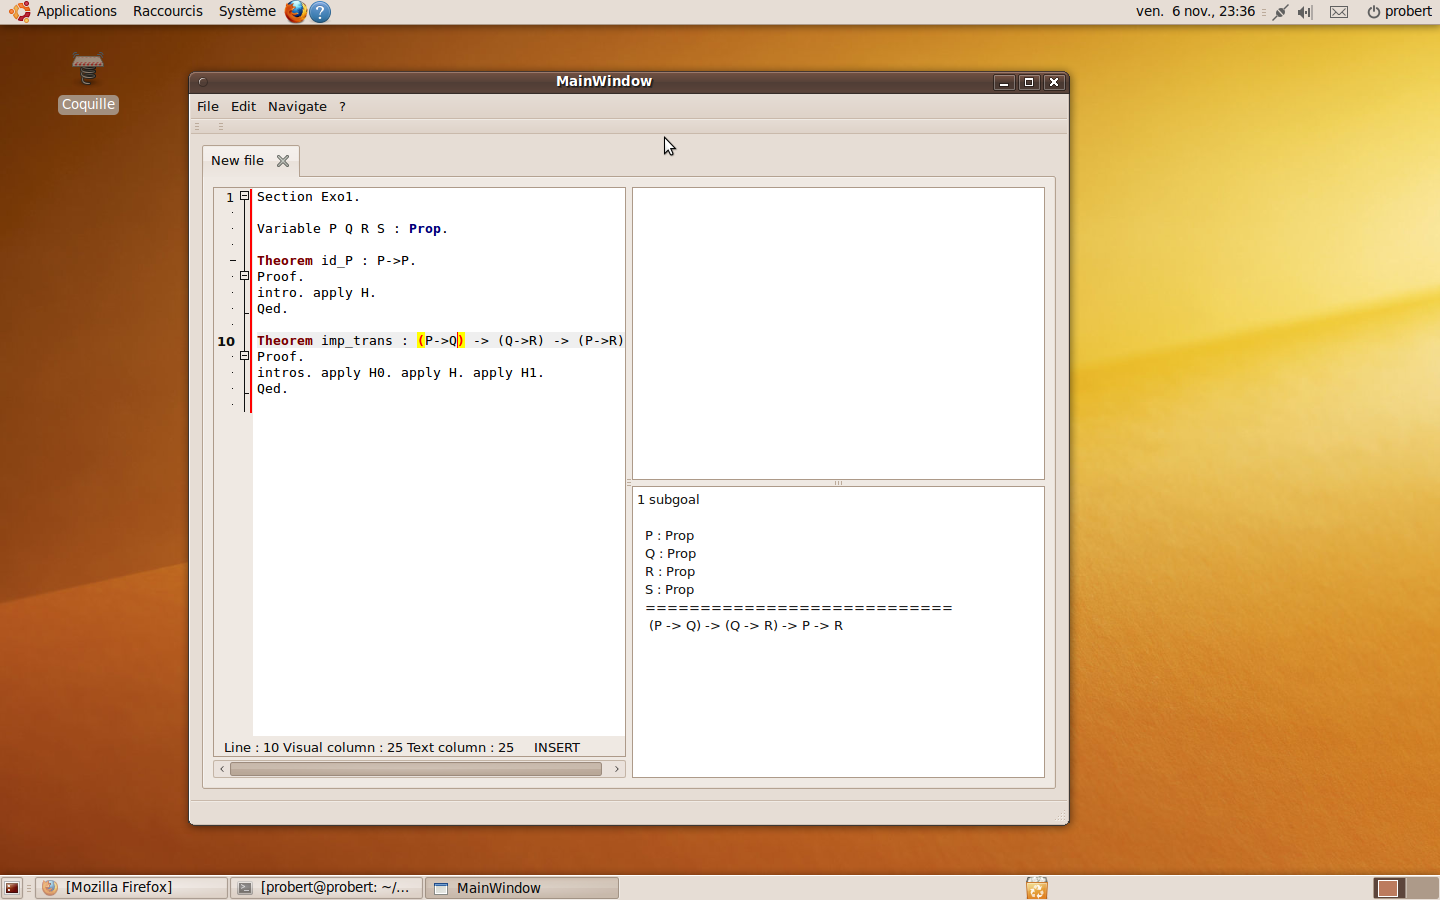
\includegraphics[scale=0.35]{Capture.png}
% Qu'est-ce qu'on fait maintenant ?
% -> on commence à penser à intégrer ce que font les autres ? Comment on va pouvoir proposer des tactiques ou de l'apprentissage ?

\section{Workpackage Apprentissage}
\paragraph{Dirigé par Guillaume Aupy}, 6 participants

\subsection{Objectifs}
L'objectif de ce groupe de travail est d'à partir de nombreux exercices, de créer des tactiques spécifiques à ce type d'exercice.

\subsection{Matériels et méthodes}
On utilise un arbre de décision. A chaque noeud de l'arbre de décision se trouve une question portant sur les arbres syntaxiques des hypothèses et du but. Pour la première question, on ne s'autorise à interroger que les racines. Ensuite, on s'autorise à interroger les fils des arbres déjà interrogés. Les questions sont "quel est le token à la racine de l'arbre x?" et "est-ce que les arbres x et y ont le même token en racine?".

Pour choisir la question à poser, on calcule la question qui nous donne le meilleur rapport "information apportée selon la définition de von Newmann" sur "nombre de réponses". On cherche donc à minimiser la taille de l'arbre (et non sa profondeur), car c'est d'elle que dépend le temps d'exécution et l'occupation de la mémoire.

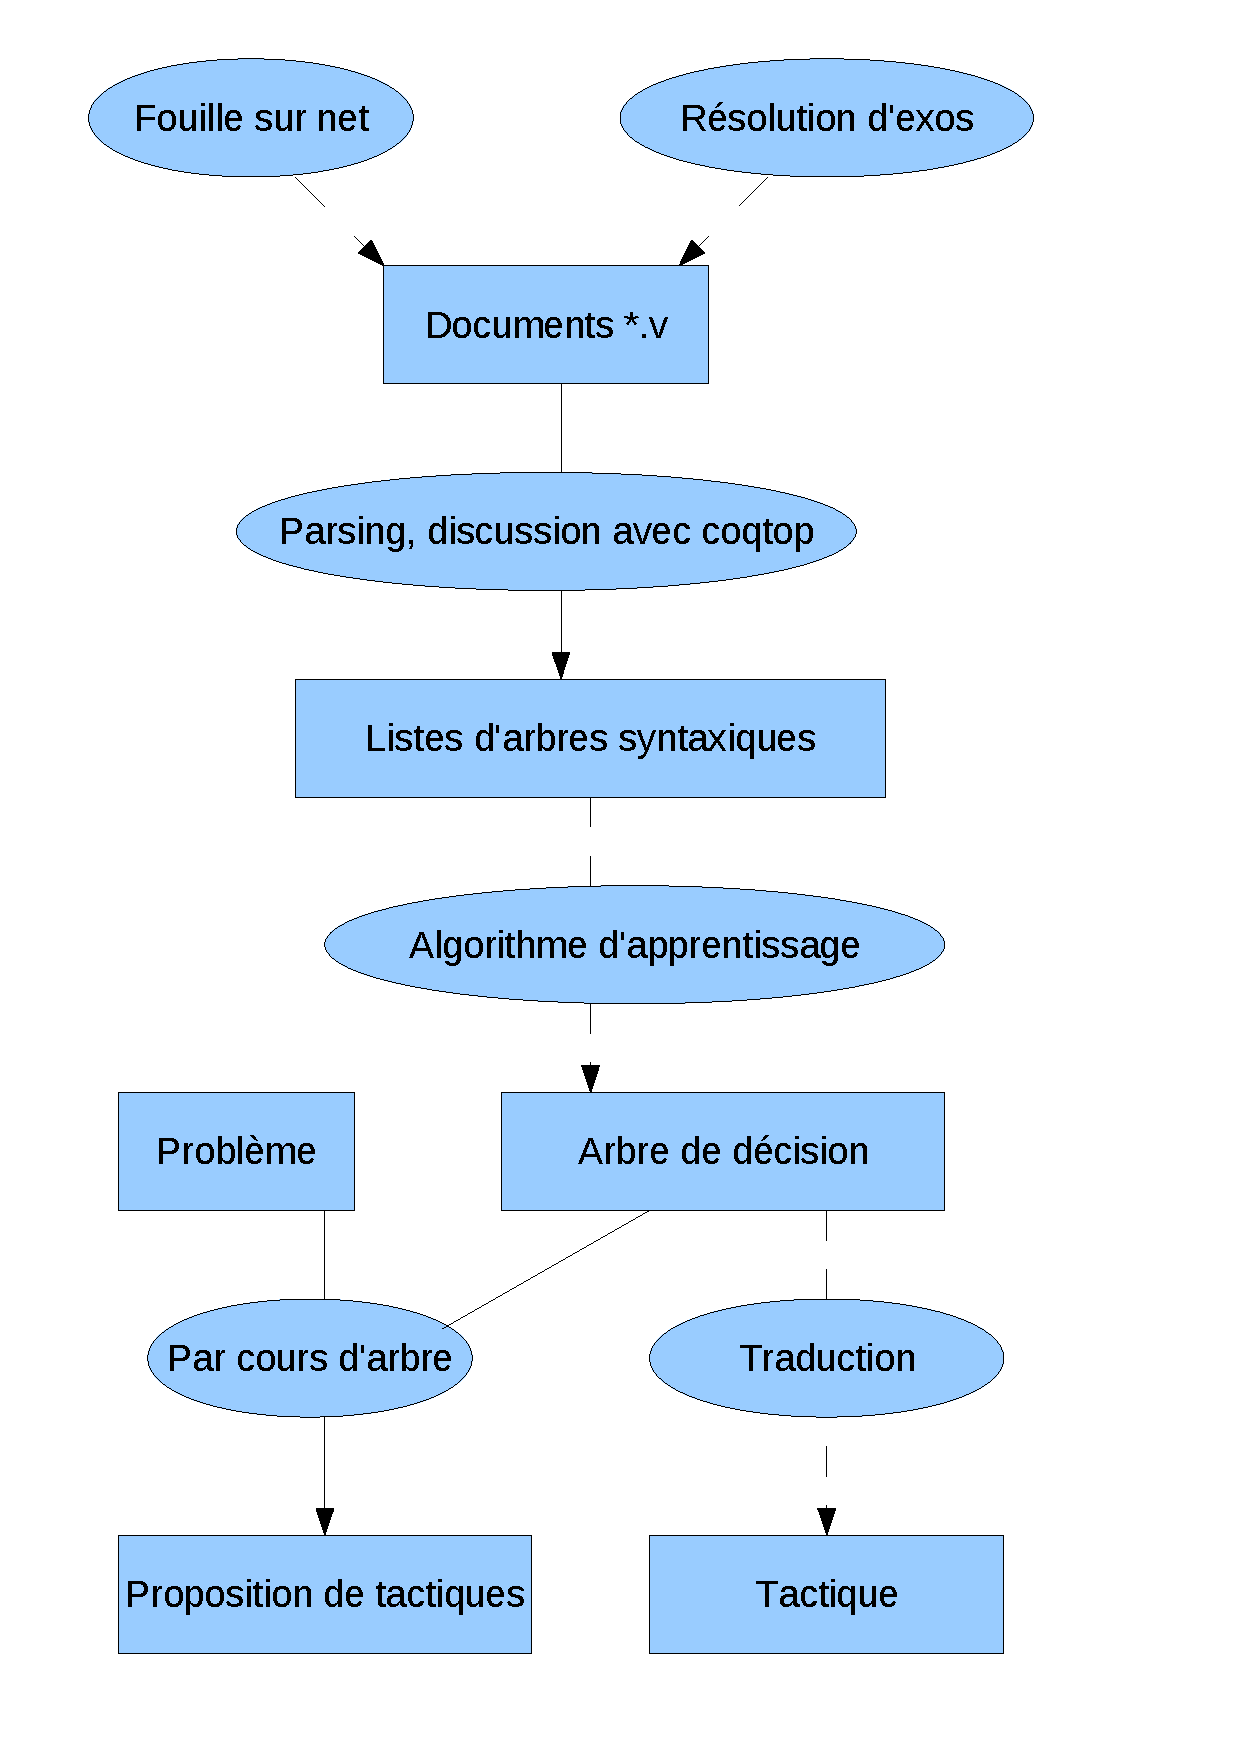
\includegraphics[scale=0.5]{organisation_apprentissage.pdf}


\subsection{Difficultés}  %à reformuler
Pour le parcours de l'abre de décision, nous avons porté une attention toute particulière à la gestion des ``choix''.
 En effet, comme il y a plusieurs hypothèses, lorsqu'on demande "quel est la racine de l'hypothèse", on fait un choix. 
Pour plus d'efficacité, on repousse ce choix au plus loin : on passe plusieurs choix possibles.
Les bonnes représentations sont essentielles car elles permettent d'éliminer les choix caduques, 
les choix dépendant d'autres choix. \\

Pour l'algorithme d'apprentissage, nous travaillons beaucoup à avoir une complexité correcte.
 Un algorithme naïf donnerait une complexité environ cubique par rapport à celle que nous avons actuellement. %à préciser

\subsection{Résultats}
Le parcours d'arbres et le rafinement des données sont utilisables (leur complexité est améliorable et des améliorations sont possibles).
 L'algorithme d'apprentissage a été réalisé, il faut maintenant le tester pour vérifier qu'il correspond bien à nos attentes.

\section{Commentaires généraux}
\subsection{Le côté pédagogique}
 Le projet reste un cours et non un projet. C'est pourquoi, nous avons préféré le côté pédagogique au côté productif. Le fait que chaque élève retienne quelquechose de cette expérience est pour nous plus important que d'être visible au niveau national.

 Nous avons donc choisi des groupes de travail très distincts, intéressant des personnes différentes. Ainsi, tous les étudiants sont motivés par le projet et s'investissent. Nous avons écarté quelques projets, certes attendu par la communauté coq, mais peu intéressant d'un point de vue pédagogique.
  Les groupes de travail IDE et Apprentissage explorent des domaines qui ne sont pas abordé lors de notre formation à l'ENS. Pourtant, il y a une forte attente dans ces domaines. Ici, le projet vient en complément de la formation, pour répondre à la curiosité des étudiants.

\subsection{La marge au niveau des objectifs}
Il est assez difficile de mesurer l'avancement du projet par rapport aux objectifs. En effet, dans chaque groupe de travail, l'objectif minimal est facilement atteignable. A mi-projet, il y a déjà un algorithme d'apprentissage basique, un environnement fonctionnel, et de nombreux théorêmes. Les objectifs sont définis en tant que ``le plus''. On cherche à avoir l'algorithme d'apprentissage le plus efficace possible, le plus de fonctionnalités possibles dans l'IDE, la bibliothèque de théorême la plus complète possible.

C'est globalement une bonne chose. Si l'objectif avait été très précis, une fois atteint il n'y aurait plus rien à faire. Ici, le groupe a déjà produit de nombreux résultats, mais continue d'avancer car il n'est pas borné par un objectif prédéfini.

\subsection{La non dépendance des groupes de travail}
Les groupes sont totalement indépendants les uns des autres, même si ils concourent au même logiciel. Un mauvais algorithme d'apprentissage n'handicape pas l'environnement et vice-versa. Cela rend la gestion du projet plus facile. Si un groupe avance moins vite faute de personne, ou parce que l'objectif est plus dur, nous ne sommes pas obligé de redistribuer les forces. Si il est préferable d'avoir des groupes de travail équilibrés, ce n'est pas une obligation. Les élèves travaille donc sur des domaines qui leur plaisent, pas forcément sur ``la tâche la plus urgente''.


\section{Bibliographie}
\begin{itemize}
\item [1] http://coq.inria.fr/stdlib/ [la coq standard library]
\item [2] http://c-corn.cs.ru.nl/documentation/toc.html% [les modules disponibles dans Corn]
\item [3] http://graal.ens-lyon.fr/coquille/
\item [4] http://perso.ens-lyon.fr/jeanmarie.madiot/coquille/forum
\item [5] http://coquille.wikispot.org/
\item [6] Artifical intelligence, a modern approach, S. Russel P. Norvig

\end{itemize}

%Les livres de classes préparatoires \\
%Les bibliothèques IDE : 

\end{document}

